\documentclass[10pt]{article}
\usepackage{url}
\usepackage{geometry}
\usepackage{booktabs}
\usepackage{graphicx}

\title{Practical backpropagation revision}
\author{Rafael}
\date{\today}

\begin{document}

\maketitle

\abstract{Based on Matt Mazur weblog}

\section{Introduction}
There are quite a number of scientific articles that detail the formalities of artificial neural networks (ANNs).
While some background knowledge about derivatives (gradiend descent), chain rule, and vector algebra is arguably enough to understand the nuts and bolts of the training of ANNs, there are underlying aspects that could remain obscure to grasp for some readers.

This document is focused on starting on a specific example of an ANN for its training and testing. 
Based on the Matt Mazur's weblog\footnote{\url{https://mattmazur.com/2015/03/17/a-step-by-step-backpropagation-example/}}, we go a beyond and provide both the practical and technical background to integrally understand the process.

The rest of this document employs the nomenclature shown in Table~\ref{tab:symbols}.

\begin{table}
%\resizebox{\textwidth}{!}{%
\begin{tabular}{@{}p{0.2\textwidth}p{0.8\textwidth}@{}}
\toprule
\textbf{Symbol} & \textbf{Meaning} \\ \midrule
$L$ & The number of layers of the feedforward multilayer network \\
$w_{ji}^{(l)}$ & The individual weight in layer $l$ coming from neuron $i$ that arrives to the neuron $j$ of layer $(l+1)$. \\ 
$v_j^l$ & The local field ($net$) of a given network. This is the dot product between the activations and weights coming from neurons of the immediate previous layer. \\
$\varphi$ & The activation (squash) function applied to the local field (\emph{net}) of a neuron. Let it be the sigmoid function. \\
$\varphi(v_j^l)$ & The output of the neuron $j$ of layer $l$. \\
...& ...\\
\bottomrule
\end{tabular}%
\caption{Symbols employed on the description}
\label{tab:symbols}
%}
\end{table}

\section{Sample ANN architecture}

\begin{figure}
	\centering
	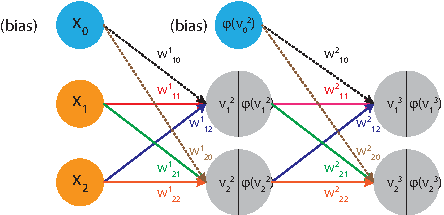
\includegraphics[scale=1.3]{figures/base-ann}
	\caption{The sample ANN to be employed during this tutorial}
	\label{fig:sample-ann}
\end{figure}

Figure~\ref{fig:sample-ann} shows the sample ANN architecture that will be employed during this tutorial.
Notice the following:
\begin{itemize}
	\item This is a 2-2-2 architecture, since there are two inputs (or attributes), two neurons in a hidden layer, and two neurons in the output layer.
	\item The employed notation allows to see that indexing could be employed for easily referencing each weight, local field ($v$) and activation $\varphi$. 
	\item Biases are represented with a 0 subindex (the top separated circles). Biases are included in the calculation of the local field $v$.
	\item There are initial values for input ($x$) and weights ($w$). We will thoroughly employ them in the following description.
	\item ...
\end{itemize}

\section{Feedforward stage}
If you have arrived to this step, presumably you known some of the following points:
\begin{itemize}
	\item The \emph{heavy} work of an ANN is carried out by the set of \emph{weights}.
	\item You can use different input data $x$ but they are actually somehow fixed.
	\item The performance of the ANN is modified by the adjustments the weights.
	\item Somehow, every labeled example-pattern should improve the performance of the ANN; as a result, somehow the errors found should modify the weights.
	\item The derivative could be employed as a way to determine whether weight values should be increased-reduced; this is linked to the gradient descend algorithm.
\end{itemize}

The rest of this section will try to describe the feedforward step, on which we evaluate the performance (accuracy) of the network predictions in order to later perform the weights adjustments (backpropagation).

\end{document}